% !TEX root = ../beamer.tex
\section{Preliminary}

\subsection{Cloud Manufacturing}
\begin{frame}{Ecosystem Main Structure}{Cloud Manufacturing}
\only<1>{
	\begin{figure}
	\centering
	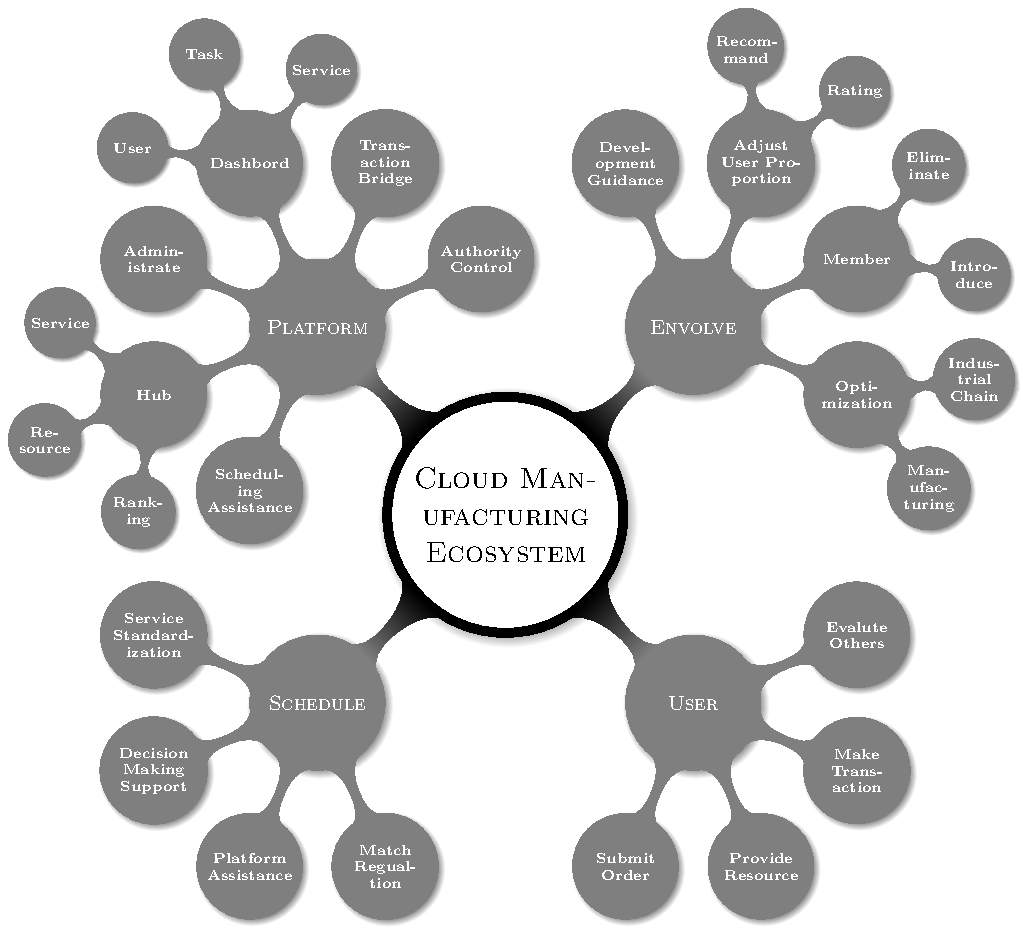
\includegraphics[height=0.82\textheight]{figures/platformstruct.pdf}
	\caption{Princiapl Structure of Cloud Manufacturing Ecosystem}
	\end{figure}
}
\iffalse
\only<2>{
	\begin{figure}
	\centering
	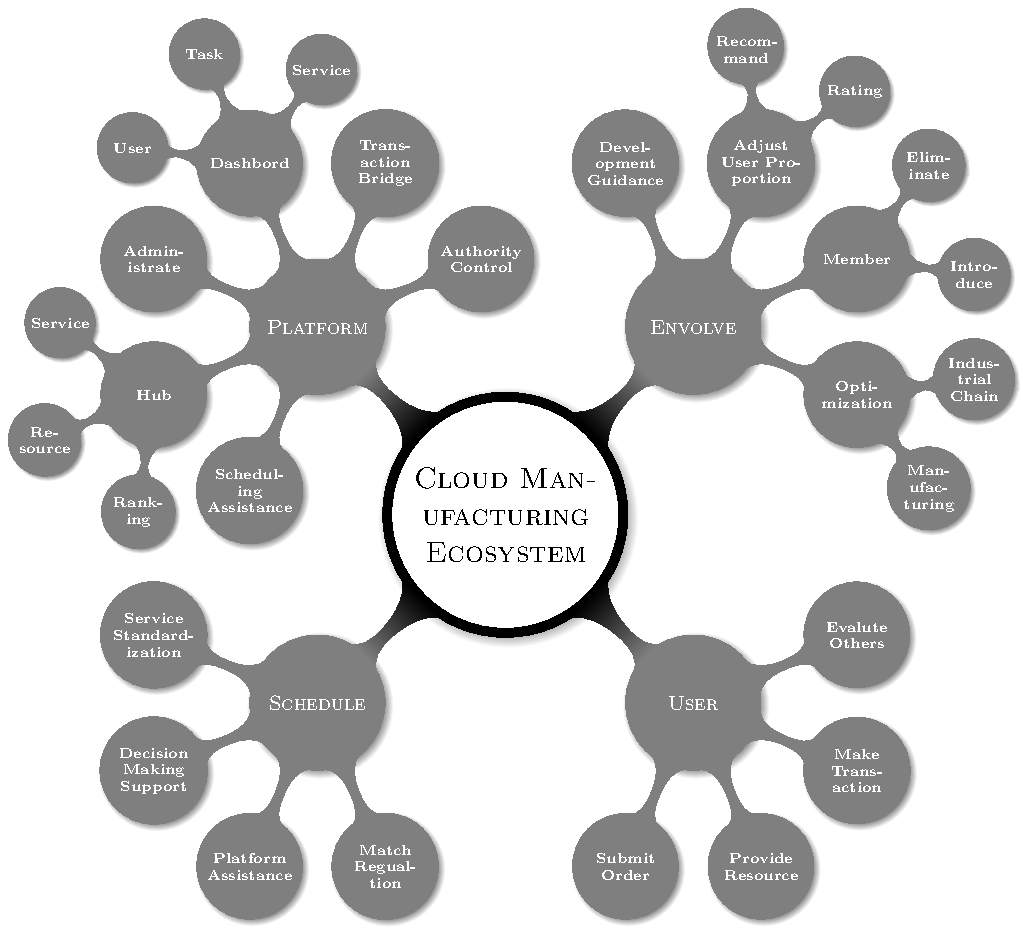
\includegraphics[height=0.82\textheight,viewport=40 0 500 250,clip=true]{figures/platformstruct.pdf}
	\end{figure}
}
\only<3>{
	\begin{figure}
	\centering
	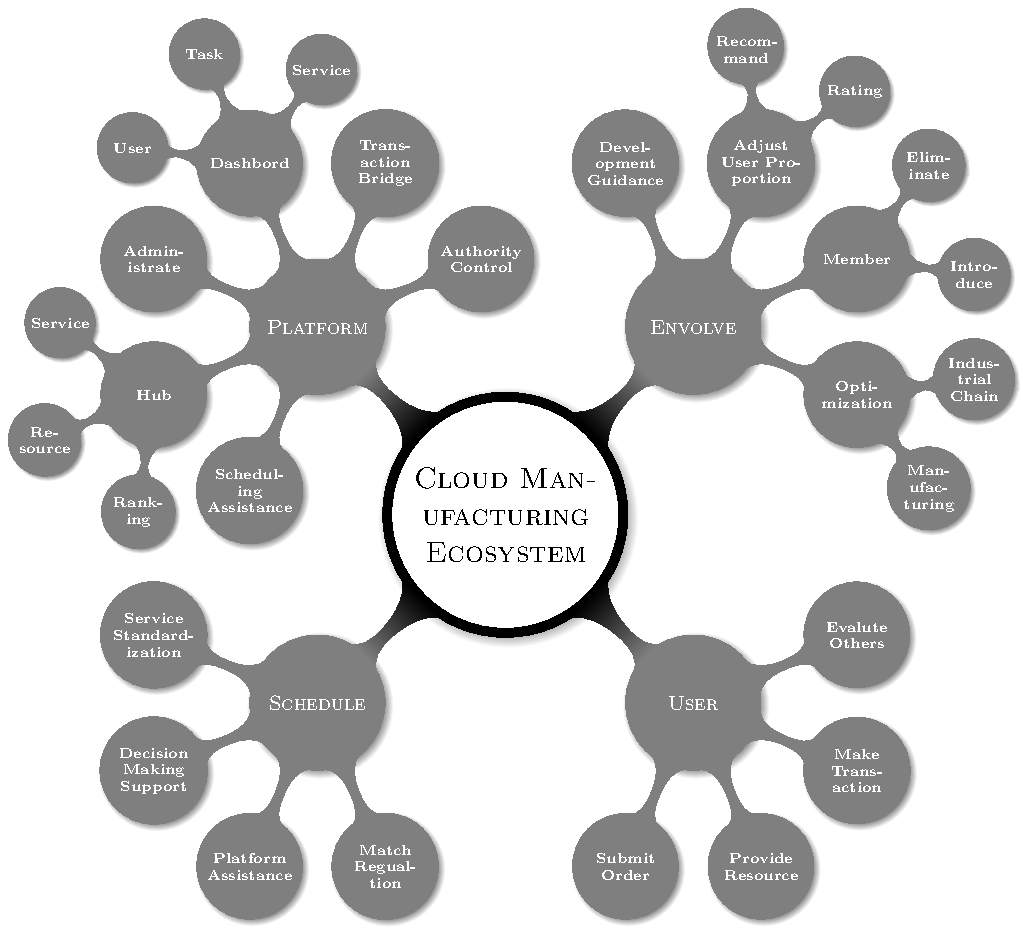
\includegraphics[height=0.82\textheight,viewport=0 160 500 450,clip=true]{figures/platformstruct.pdf}
	\end{figure}
}
\fi
\end{frame}

\begin{frame}{Service Standardization}{Cloud Manufacturing}
\begin{figure}
\centering
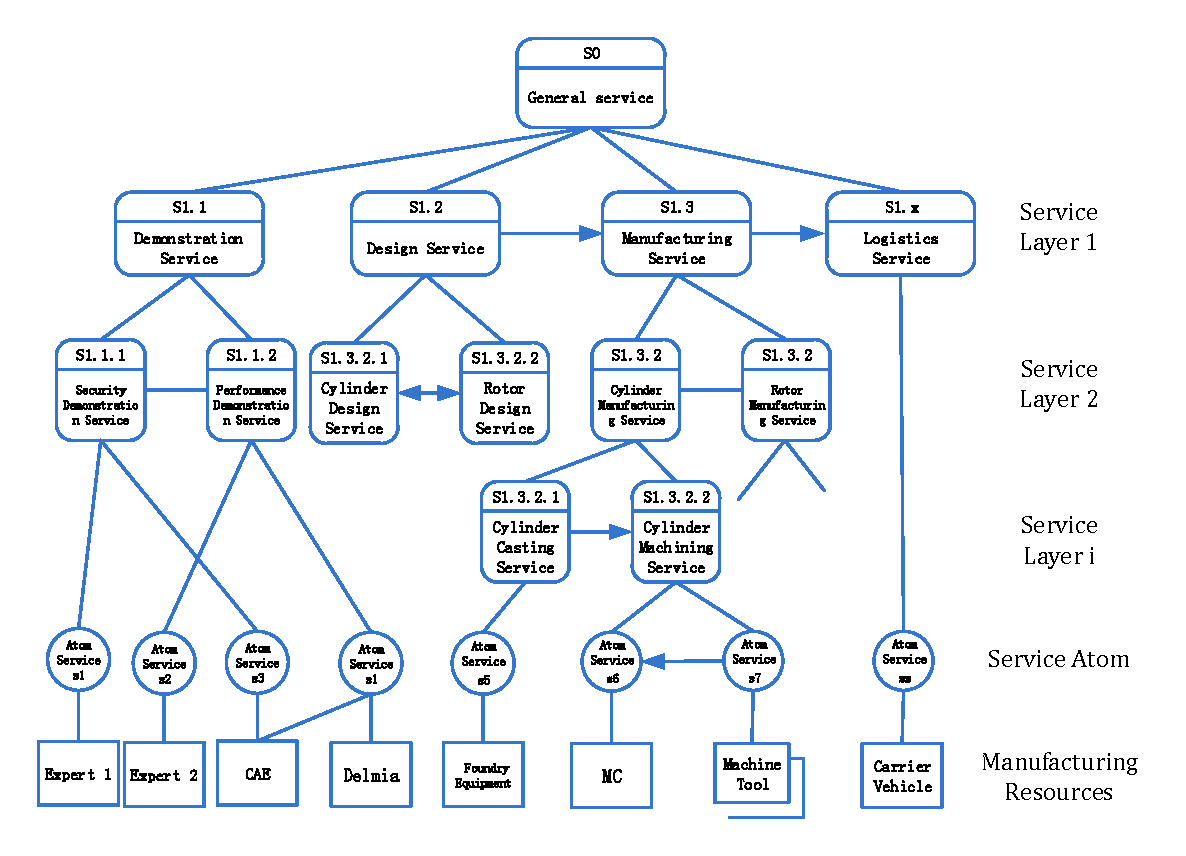
\includegraphics[height=0.85\textheight]{figures/boss.pdf}
\caption{Standard Service Tree Illustration}
\end{figure}
\iffalse
\onslide<+->{
	Cloud Manufacturing Ecosystem provides a platform which distributed manufacturing resources/orders gathered as resources/orders hub. 
}
\onslide<+->{
	\begin{block}{Related Methods}
	\begin{itemize}
	\item Resource Virtualization
	\item Construct Virtual Resource into Service Unit
	\item Service Standardization
	\item Order Decomposition into Tasks
	\end{itemize}
	\end{block}
}
\fi
\end{frame}

\subsection{Roles}
\begin{frame}{Usual Names}{Roles}
\onslide<+->{\small
	\begin{description}
	\item[User] The main role in Cloud Manufacturing, usually acts as Seller or Buyer;
	\item[Seller] The temporary role in a transaction, which provides the allocated part of manufacturing service;
	\item[Buyer] The temporary role in a transaction, which submits the allocated part of manufacturing task;
	\item[Administrator] The role that gets the work for the operation and maintenance of the platform.
	\end{description}
}
\onslide<+->{
\begin{table}[htbp]
  \centering\scriptsize
    \begin{tabular}{lcc}
    \toprule
        &  Seller & Buyer  \\
    \midrule
    Generalized User & $\surd$ & $\surd$  \\
    Enterprise User & $\surd$ &  \\
    Customer User& & $\surd$ \\
    \bottomrule
    \end{tabular}%
\end{table}
}
\end{frame}

\subsection{Operating Model}
\begin{frame}{Overview}{Operating Model}
\only<1>{The style the Cloud Manufacturing Ecosystem appears mainly depends on the way the operating model takes, therefore, research on features and issues in the Ecosystem would be taken within the scope of operating model we are going to set up in:
\begin{block}{Operating Model Components}
\begin{itemize}
\item Order Flow
\item User Rank
\item Platform
\end{itemize}
\end{block}}
\only<2>{\begin{figure}
\tiny\centering\resizebox{\textwidth}{!}{
% !TEX root = flow_head.tex
\begin{tikzpicture}[
 >=triangle 60,              % Nice arrows; your taste may be different
 start chain=going right,    % General flow is top-to-bottom
 node distance=12em and 3em, % Global setup of box spacing
 every join/.style={norm},   % Default linetype for connecting boxes
]
% ------------------------------------------------- 
% A few box styles 
% <on chain> *and* <on grid> reduce the need for manual relative
% positioning of nodes
\tikzset{
  every node/.style={rectangle split, rectangle split parts=2, rectangle split horizontal, rectangle split part fill={lccong!25, yellow!10}, draw, anchor=center, minimum height=9em, on chain, on grid, text width=2em},
  base/.style={draw, on chain, on grid, align=center, minimum height=4ex},
  proc/.style={base, rectangle, text width=8em},
  Arrow/.style={thick, decoration={markings,mark=at position
   1 with {\arrow[semithick]{open triangle 60}}},
   double distance=1.4pt, shorten >= 5.5pt,
   preaction = {decorate},
   postaction = {draw,line width=1.4pt, white,shorten >= 4.5pt},fill = lcnorm!25},
  test/.style={base, diamond, aspect=2, text width=5em},
  term/.style={proc, rounded corners},
  % coord node style is used for placing corners of connecting lines
  coord/.style={coordinate, on chain, on grid, node distance=6mm and 25mm},
  % nmark node style is used for coordinate debugging marks
  nmark/.style={draw, cyan, circle, font={\sffamily\bfseries}},
  % -------------------------------------------------
  % Connector line styles for different parts of the diagram
  norm/.style={->, draw, lcnorm, thick},
  free/.style={->, draw, lcfree},
  cong/.style={->, draw, lccong},
  it/.style={font={\small\itshape}},
  tw/.style={text width=9.5em},
  th/.style={text width=2em}
}

\newcommand{\one}[1]{\nodepart[th]{one}\rotatebox{90}{\bf\shortstack{#1}}}
\newcommand{\two}{\nodepart[tw]{two}}

\node (n1)
{	
	\one{Service\\ Provide}
	\two
	\begin{inparaenum}
	\item 1.Submit Resources\\
	\item 2.Construct Resources into Services\\
	\item 3.Service Standardization
	\end{inparaenum}
};

\node[join] (n2) 
{
	\one{Task\\ Matching}
	\two
	\begin{inparaenum}
	\item 1.Recommanded Tasks\\
	\item 2.Order Acception \\
	\item 3.Decision
	\end{inparaenum}
};

\node[join] (n3)
{
	\one{Manufacturing\\ \& Schedule}
	\two
	\begin{inparaenum}
	\item 1.Manufacturing\\
	\item 2.Schedule Tasks\\
	\item 3.Outsourcing\\
	\item 4.Receive job pieces
	\end{inparaenum}
};

\node[below=of n3,join] (n4)
{
	\one{Delivery}
	\two
	\begin{inparaenum}
	\item 1.Deliver Completed job\\
	\item 2.Wait for Confirmation
	\end{inparaenum}
};

\node[below=of n2,join] (n5)
{
	\one{Mutual\\ Rating}
	\two
	\begin{inparaenum}
	\item 1.Rate Buyer\\
	\item 2.Receive Rate by Buyer\\
	\item 3.Change Rank\\
	\item 4.Change Recommendation
	\end{inparaenum}
};
\end{tikzpicture}}
\caption{Seller Flow in Operating Model}
\end{figure}}
\only<3>{\begin{figure}
\tiny\centering\resizebox{\textwidth}{!}{
% !TEX root = flow_head.tex
\begin{tikzpicture}[
 >=triangle 60,              % Nice arrows; your taste may be different
 start chain=going right,    % General flow is top-to-bottom
 node distance=12em and 3em, % Global setup of box spacing
 every join/.style={norm},   % Default linetype for connecting boxes
]
% ------------------------------------------------- 
% A few box styles 
% <on chain> *and* <on grid> reduce the need for manual relative
% positioning of nodes
\tikzset{
  every node/.style={rectangle split, rectangle split parts=2, rectangle split horizontal, rectangle split part fill={lccong!25, yellow!10}, draw, anchor=center, minimum height=9em, on chain, on grid, text width=2em},
  base/.style={draw, on chain, on grid, align=center, minimum height=4ex},
  proc/.style={base, rectangle, text width=8em},
  Arrow/.style={thick, decoration={markings,mark=at position
   1 with {\arrow[semithick]{open triangle 60}}},
   double distance=1.4pt, shorten >= 5.5pt,
   preaction = {decorate},
   postaction = {draw,line width=1.4pt, white,shorten >= 4.5pt},fill = lcnorm!25},
  test/.style={base, diamond, aspect=2, text width=5em},
  term/.style={proc, rounded corners},
  % coord node style is used for placing corners of connecting lines
  coord/.style={coordinate, on chain, on grid, node distance=6mm and 25mm},
  % nmark node style is used for coordinate debugging marks
  nmark/.style={draw, cyan, circle, font={\sffamily\bfseries}},
  % -------------------------------------------------
  % Connector line styles for different parts of the diagram
  norm/.style={->, draw, lcnorm, thick},
  free/.style={->, draw, lcfree},
  cong/.style={->, draw, lccong},
  it/.style={font={\small\itshape}},
  tw/.style={text width=9.5em},
  th/.style={text width=2em}
}

\newcommand{\one}[1]{\nodepart[th]{one}\rotatebox{90}{\bf\shortstack{#1}}}
\newcommand{\two}{\nodepart[tw]{two}}

\node (n1)
{	
	\one{Submit\\ Order}
	\two
	\begin{inparaenum}
	\item 1.Original\\
	\item 2.Outsourcing
	\end{inparaenum}
};

\node[join] (n2) 
{
	\one{Task\\ Construct}
	\two
	\begin{inparaenum}
	\item 1.Order Decomposition\\
	\item 2.Task Merging\\
	\item 3.Task Splitting
	\end{inparaenum}
};

\node[join] (n3)
{
	\one{Service\\ Matching}
	\two
	\begin{inparaenum}
	\item 1.Recommandation\\
	\item 2.Service Selection\\
	\item 3.Seller's Rank
	\end{inparaenum}
};

\node[below=of n3,join] (n4)
{
	\one{Confirm\\ by Seller}
	\two
	\begin{inparaenum}
	\item 1.Accept Tasks\\
	\item 2.Check Due-date\\
	\item 3.Buyer Rank
	\end{inparaenum}
};

\node[below=of n2,join] (n5)
{
	\one{Wait for\\ Delivery}
	\two
	\begin{inparaenum}
	\item 1.Wait the Seller\\
	\item 2.Confirm the Prouct\\
	\item 3.Pay for it
	\end{inparaenum}
};

\node[below=of n1,join] (n6)
{
	\one{Mutual\\ Rating}
	\two
	\begin{inparaenum}
	\item 1.Rate Seller\\
	\item 2.Change Rank\\
	\item 3.Affect Recommand
	\end{inparaenum}
};
\end{tikzpicture}}
\caption{Buyer Flow in Operating Model}
\end{figure}}
\end{frame}

\begin{frame}{Order Flow}{Operating Model}
\only<1>{Each order appears when Users make transaction in the platform, it might then go through different paths:
\begin{figure}
\tiny\centering
%\resizebox{\textwidth}{!}{% !TEX root = flow_head.tex
\begin{tikzpicture}[%
    >=triangle 60,              % Nice arrows; your taste may be different
    start chain=going below,    % General flow is top-to-bottom
    node distance=6mm and 60mm, % Global setup of box spacing
    every join/.style={norm},   % Default linetype for connecting boxes
    ]
% ------------------------------------------------- 
% A few box styles 
% <on chain> *and* <on grid> reduce the need for manual relative
% positioning of nodes
\tikzset{
  base/.style={draw, on chain, on grid, align=center, minimum height=4ex},
  proc/.style={base, rectangle, text width=8em},
  test/.style={base, diamond, aspect=2, text width=5em},
  term/.style={proc, rounded corners},
  % coord node style is used for placing corners of connecting lines
  coord/.style={coordinate, on chain, on grid, node distance=6mm and 25mm},
  % nmark node style is used for coordinate debugging marks
  nmark/.style={draw, cyan, circle, font={\sffamily\bfseries}},
  % -------------------------------------------------
  % Connector line styles for different parts of the diagram
  norm/.style={->, draw, lcnorm},
  free/.style={->, draw, lcfree},
  cong/.style={->, draw, lccong},
  it/.style={font={\small\itshape}}
}
% -------------------------------------------------
% Start by placing the nodes
\node [term] {Be Submitted};
\end{tikzpicture}
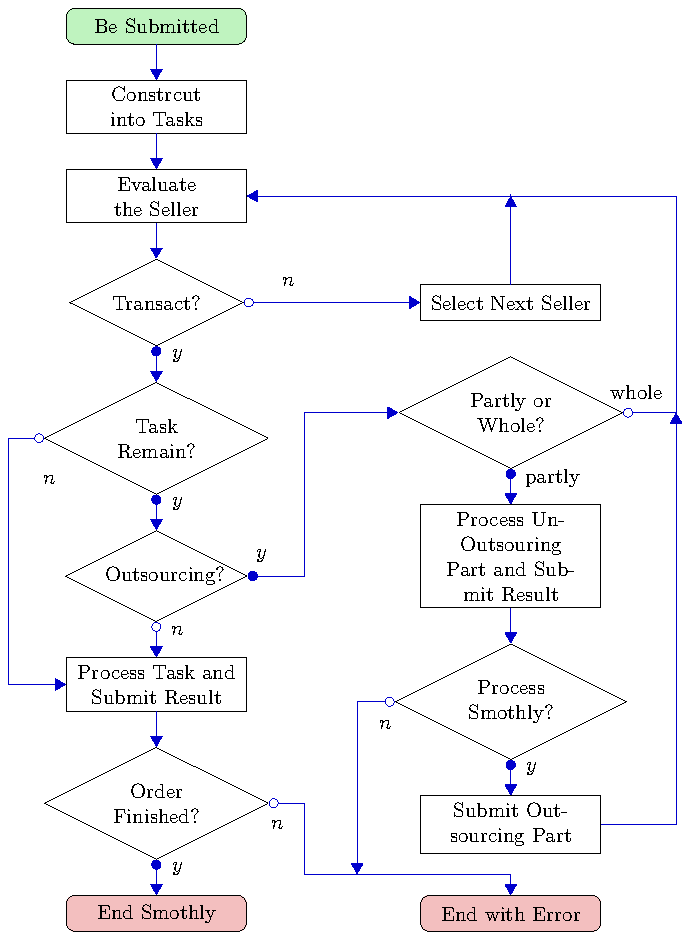
\includegraphics[height=0.9\textheight,angle=90]{figures/orderflow.pdf}
%}
\caption{Simple Flow Chart of Order}
\end{figure}
}
\end{frame}

\begin{frame}{User Rank}{Operating Model}
\onslide<+->{User Rank provides the basis to make the recommandation and to get more permission, the rank will increase or decrease by good or bad performance in each transaction}
\onslide<+->{
\begin{equation}
  \begin{cases}
      Rank_{[T+1]} = Rank_{[T]} + Gain - Lose, & T \geqslant 1\\
      Rank_{[0]} = Rank_{[init]}
  \end{cases}
\end{equation}
}
\end{frame}

\begin{frame}{Platform}{Operating Model}
\onslide<+->{
	Cloud Manufacturing Platform is mantained by Administrators with:
}
\onslide<+->{
	\begin{block}{Platform Maintenances}
	\begin{itemize}
	\item Decompose Orders into Tasks
	\item Construct Standard Services
	\item Introduce/Eliminate Users
	\item Distribute Permissions
	\item Adjust Resource Useage by Recommandations and Bonus
	\end{itemize}
	\end{block}
}
\end{frame}

\subsection{Data Science Tools}
\begin{frame}{Data Science Tools}
\onslide<+->{In such Cloud Manufacturing Operating Model, there comes massive amount of data:\begin{itemize}
  \item Transaction histroy;
  \item Ranking histroy;
  \item Status of resources, services, orders and tasks;
  \item Decision pattern and so on.
\end{itemize}}
\onslide<+->{
	A bunch of Data Science Tools can be helpful:
	\begin{block}{Useful Data Science Tools}
	\begin{itemize}
	\item Data Analysis (collection, cleaning, modeling\&algorithms)
	\item Data Warehousing
	\item Machine Learning
	\item Social Network Anaysis
	\end{itemize}
	\end{block}
}
\end{frame}

%\begin{frame}{Blocks}
%\begin{block}{Block Title}
%You can also highlight sections of your presentation in a block, with it's own title
%\end{block}
%\begin{theorem}
%There are separate environments for theorems, examples, definitions and proofs.
%\end{theorem}
%\begin{example}
%Here is an example of an example block.
%\end{example}
%\end{frame}

% Placing a * after \section means it will not show in the
% outline or table of contents.
